\section{Applying the Best Classifiers}
\label{subsection:applying-classifiers}

A novel approach is now introduced to determine which of the top models perform best in a simulation of a real life scenario. 

\subsection{Scenario Overview}
A classifier will be used to batch process a corpus of previously unseen questions, called \verb|dataset_02|, to determine whether or not they are bullying in nature. The predictions, bullying or not bullying, from each batch of questions processed, are then fed back into the training dataset and a new model is generated. The next batch of questions is then classified. This process continues until all samples have been processed. 

A third test dataset, \verb|dataset_03|, never used at any point in the development of any of the classifiers, will be used to gauge the performance of each of the models before and after the batch processing, in order to determine which model produced the best classifier.

The steps to achieve this can be summarised as follows:

\begin{itemize}

	\item Prepare the two datasets put aside for this testing in Chapter \ref{chapter4} by generating NLTK or Scikit-Learn corpora as required.
	\item Classify both datasets using the three top models and record the performance results.
	\item Simulate the growth in each of the models using \verb|dataset_02|.
	\item Re-evaluate \verb|dataset_03| again using each of the final models and see if the models performance has increased or decreased. Also compare the complete set of before and after results from \verb|dataset_02|.

\end{itemize}

\subsection{Data Preparation}
At the end of Chapter \ref{chapter4} \verb|dataset_02| and \verb|dataset_03| had not been preprocessed or stored in the correct corpora format for NLTK or Scikit-Learn. In a real life scenario, the processing required to do this would all have to happen as the data is received. However, in this simulation, all preparatory work was performed upfront. Each dataset was first preprocessed and cleansed using the same Python script as described in Section \ref{section:data_prepatation}. Next, each dataset was saved in the basic NLTK corpus format and renamed as \verb|sim_01| and \verb|hb_01|. The NLTK models to be tested required the dataset in bi-gram and tri-gram format, and with and without stop words removed. This produced eight further NLTK corpora called \verb|sim_02|, \verb|sim_03|, \verb|sim_12|, \verb|sim_13|, \verb|hb_02|, \verb|hb_03|, \verb|hb_12| and \verb|hb_13|. Both of the Scikit-Learn models used the NLTK \verb|sim_01| and \verb|hb_01| corpora but with all the samples presented in a single comma separated file format as before.

\subsection{Initial Analysis}
It would not be feasible, at this stage, to fully evaluate all 24 models identified for further analysis. In order to reduce the number, an initial simple analysis was performed whereby all unseen samples in the simulation and hold-back datasets were classified, and the percentage of bullying questions predicted was calculated. In Table \ref{tab:chapter5:simple_initial_analysis} the 24 models being evaluated are listed. First, on the left-hand side, they are listed by g-performance and then, on the right-hand side, in the percentage of bullying questions each model found. When manually classifying the training data, the percentage of bullying questions identified was 15.17\%. This is also shown in the table. To proceed to the next phase, it was necessary to identify the models with the best potential to generalise to the population. 

\begin{table}[h]
\centering
\caption[Simple performance measurement of top 24 models]{Table showing the top 24 models sorted by g-performance, left-hand side, and percentage of unseen data predicted as bullying, right-hand side}
\label{tab:chapter5:simple_initial_analysis}
\begin{tabular}{rccrlrcc}
	\toprule
	\multicolumn{3}{c}{\textbf{Sort By G-Performance}} & \multicolumn{2}{c}{\textbf{ }} & \multicolumn{3}{c}{\textbf{Sort By Predicted Bullying}} \\
	\cmidrule(r){1-3}
	\cmidrule(r){6-8}
	\textbf{Ref:} & \textbf{Bullying} & \textbf{G-Perf} & \multicolumn{2}{c}{\textbf{ }} & \textbf{Ref:} & \textbf{Bullying} & \textbf{G-Perf} \\
    \midrule
	1 & 2.34\% & 0.9920 &  &  & 16 & 29.69\% & 0.8547 \\
	9 & 2.50\% & 0.9918 &  &  & 15 & 27.94\% & 0.8649 \\
	2 & 2.32\% & 0.9918 &  &  & 8 & 25.30\% & 0.8681 \\
	10 & 2.36\% & 0.9916 &  &  & 7 & 24.84\% & 0.8687 \\
	17 & 15.51\% & 0.9508 &  &  & 23 & 23.44\% & 0.9170 \\
	3 & 12.74\% & 0.9448 &  &  & 21 & 17.87\% & 0.9210 \\
	11 & 13.43\% & 0.9418 &  &  & 14 & 17.80\% & 0.9199 \\
	18 & 13.49\% & 0.9399 &  &  & 13 & 16.82\% & 0.9256 \\
	4 & 13.56\% & 0.9390 &  &  & 22 & 16.65\% & 0.9196 \\
	12 & 14.98\% & 0.9369 &  &  & 6 & 16.03\% & 0.9225 \\
    \midrule
	\rowcolor{LightCyan}
	19 & 10.04\% & 0.9357 &  &  & 17 & 15.51\% & 0.9508 \\
	\rowcolor{LightCyan}
	5 & 15.32\% & 0.9288 &  &  & 5 & 15.32\% & 0.9288 \\
	\rowcolor{LightCyan}
	&&&&&&\textbf{15.17}\%& \\
	\rowcolor{LightCyan}
	13 & 16.82\% & 0.9256 &  &  & 12 & 14.98\% & 0.9369 \\
	\rowcolor{LightCyan}
	20 & 14.30\% & 0.9240 &  &  & 20 & 14.30\% & 0.9240 \\
	\rowcolor{LightCyan}
	6 & 16.03\% & 0.9225 &  &  & 24 & 13.58\% & 0.8945 \\
    \midrule
	21 & 17.87\% & 0.9210 &  &  & 4 & 13.56\% & 0.9390 \\
	14 & 17.80\% & 0.9199 &  &  & 18 & 13.49\% & 0.9399 \\
	22 & 16.65\% & 0.9196 &  &  & 11 & 13.43\% & 0.9418 \\
	23 & 23.44\% & 0.9170 &  &  & 3 & 12.74\% & 0.9448 \\
	24 & 13.58\% & 0.8945 &  &  & 19 & 10.04\% & 0.9357 \\
	7 & 24.84\% & 0.8687 &  &  & 9 & 2.50\% & 0.9918 \\
	8 & 25.30\% & 0.8681 &  &  & 10 & 2.36\% & 0.9916 \\
	15 & 27.94\% & 0.8649 &  &  & 1 & 2.34\% & 0.9920 \\
	16 & 29.69\% & 0.8547 &  &  & 2 & 2.32\% & 0.9918 \\    
	\bottomrule
    \end{tabular}
\end{table}

There are several conclusions that can be made by reviewing the percentage of the unseen samples that were predicted as bullying. Looking first at the top 5 performing models, models 16, 15, 8, 7 and 23, each has classified over 20\% of the questions as bullying. As the manually classified samples only had 15.17\% cyberbullying content, it is highly probable that these classifiers are predicting a large number of false positives. It would not be expected that such a classifier would predict a higher percentage of a minority class in this manner. A cursory examination of the questions classified as bullying confirmed this to be the case so these models were not considered further. In general, when classifying unseen data in this manner, a prediction rate similar to, or lower than, the training data is what would be expected. For this reason, and the need to reduce the number of models to be considered further, the next 5 models, 21, 14, 13, 22 and 6, were also ruled out of consideration.

At the bottom of the table it can be seen that four models performed really poorly on the unseen data. Models 9, 10, 1 and 2, all only managed to identify approximately 2.5\% of the unseen data as cyberbullying. This number appears to be unrealistically low and it was noticed that these, in fact, were the top four models when ordered by g-performance value. Further examination revealed that these were all NLTK models utilising tri-grams and the highest ratios of over sampling and hybrid sampling. This led to the conclusion that these models had been over fitted to the training data. A detailed examination was not feasible in the time available. However, the distribution of the tri-gram tokens seen in Section \ref{section:data_exploration}, where the overwhelming majority of the tokens only appeared once in the dataset, does support this conclusion that the models were over fitted. These four models were immediately rejected.

Of the remaining ten models the five with the lowest cyberbullying percentages, models 4, 18, 11, 3, 19 were also discarded leaving five models to be further examined. These models are highlighted in Table \ref{tab:chapter5:simple_initial_analysis} and are:

\begin{itemize}

	\item Scikit-Learn Support Vector with 1:1 over sampling, stop words included and uni-grams and bi-grams
	\item NLTK 1:1 Naive Bayes over sampling, stop words removed and tri-grams
	\item NLTK 50:50 Naive Bayes hybrid sampling, stop words removed and bi-grams
	\item Scikit-Learn Naive Bayes with 60:40 hybrid sampling, stop words included and uni-grams, bi-grams and tri-grams
	\item Scikit-Learn Support Vector with 70:30 hybrid sampling, stop words included and uni-grams, bi-grams and tri-grams

\end{itemize}

It was reassuring to see the variety of model types, sampling types and even stop word and n-gram differences across the five models selected. The next step is to perform the simulation of the evolution of each of these models as unseen samples are classified and then fed back into the model.

One final observation, from the analysis of Table \ref{tab:chapter5:simple_initial_analysis}, is that the top four models, sorted by g-performance, were the worst four when sorted by percentage of unseen samples classified as bullying. It was also noted that the worst four models, again when sorted by g-performance, yielded the models that gave the highest percentage of bullying samples in the unseen data. Expanding these observations further, seven out of the top ten by g-performance were in the bottom 10 by percentage predicted, and nine of the bottom ten by g-performance appeared in the top ten sorted by bullying percentage predicted. It was noted earlier that NTLK with tri-grams and stop words removed did not generalise well to the unseen data. Further examination showed that the top 4 models, when sorted by bullying percentage predicted, were all NLTK models using bi-grams and with stop words included. This may just be a coincidence, given the selection of the models and how they were sorted, but it could well be that a combination of there two types of models could prove very accurate if developed.

\subsection{Batch Processing of Samples}

Each of the five models identified were then further examined using the simulation dataset as follows:

\begin{itemize}

	\item The simulation dataset of 87,205 samples was divided into twenty distinct datasets.
	\item Then, for each of these datasets:
	
	\begin{itemize}
	
		\item The initial manually classified training dataset was loaded
		\item The training dataset was sampled as required by the model, either hybrid sampling or over sampling
		\item The model under test was recreated initially using the original training data for the first iteration. Subsequent iterations use the original training data and all simulation samples classified in the previous iterations
		\item The simulation dataset portion is classified using this model
		\item The classified simulation samples were appended to the training dataset for the next iteration
		\item Process repeated until there were no further simulation datasets 
	
	\end{itemize}
	
	\item Once all the simulation samples are included in the final model, the hold back dataset was classified and the results were written to a file.

\end{itemize}

This simple process was repeated for all models. In addition to writing the hold back classification results to file, each of the results for the classification of the simulation samples were also written to file. The results of this batch processing and classification of the hold back data was then analysed.

The goal of this exercise was to determine if the model, without any further manual intervention, would continue to correctly identify cyberbullying. There are three possible outcomes to be considered:

\begin{itemize}

	\item The model starts to under-predict cyberbullying \\
	In this case the percentage of cyberbullying samples seen in the hold-back will be significantly less than before the simulation. 
	\item The predictions from the model remain constant \\
	The percentage of hold-back cyberbullying samples predicted after the simulation is similar to what was seen before when only the manually classified samples were used to train the model.
	\item The model starts to over-predict cyberbullying \\
	Here the number of hold-back samples predicted as cyberbullying, after the simulation dataset has been processed, will greatly exceed the original number predicted.

\end{itemize}

Ideally only a small variance, when compared to the number originally predicted by each model, and to the percentage seen in the manually classified training data, will be seen.

A Python script, giving a sample implementation of this simulation, is given in Appendix \ref{app:simulation}.

\subsection{Analysis of Batch Processing Results}

Once the simulation had been run for each model the results were analysed. It was immediately obvious that both of the NLTK models appear to have over-predicted samples as cyberbullying. The NLTK Naive Bayes model using 1:1 over sampling, stop words removed and tri-grams predicted 37.2\% of the hold-back samples as bullying. The NLTK Naive Bayes model using 50:50 hybrid sampling, stop words removed and bi-grams predicted that 40.1\% of the hold-back samples were bullying. These numbers are representative of a potential significant increase in the number of false positive predictions made by the model. Taking a closer look at the number of samples predicted as bullying and not bullying, for each of the NLTK Naive Bayes models we get the figures in Table \ref{tab:chapter5:nltk_model_analysis}. The column labelled \verb|Model 02| represent the over sampling model, with \verb|Model 03| representing the hybrid sampling model.

\begin{table}[h]
\centering
\caption[NLTK Models, analysis of samples predicted]{Table showing the number of bullying, not bullying, changed and unchanged sample predictions for each of the NLTK models}
\label{tab:chapter5:nltk_model_analysis}
\begin{tabular}{llrcr}
	\multicolumn{5}{c}{\textbf{NLTK Model Analysis}}  \\
    \toprule
	\multicolumn{2}{l}{\textbf{Description }} & \textbf{Model 02} &  &  \textbf{Model 03} \\
    \midrule
	\multicolumn{2}{l}{\textbf{Total Samples}} & 9464 &  & 9331  \\
	\multicolumn{2}{l}{\textbf{Before simulation}} &  &  &   \\
	 & Bullying     & 1474 &  & 1425  \\
	 & Not Bullying & 7990 &  & 7906  \\
	\multicolumn{2}{l}{\textbf{After simulation}} &  &  &   \\
	 & Bullying     & 3519 &  & 3792  \\
	 & Not Bullying & 5945 &  & 5539  \\
	\multicolumn{2}{l}{\textbf{Unchanged}} &  &  &   \\
	 & Bullying     & 1401 &  & 1364  \\
	 & Not Bullying & 5872 &  & 5478  \\
	\multicolumn{2}{l}{\textbf{Changed}} &  &  &   \\
	 & Bullying to Not Bullying  & 73 &  & 61  \\
	 & Not Bullying  to Bullying & 2118 &  & 2428  \\
	\bottomrule
	\end{tabular}
\end{table}

Only 73 samples in \verb|Model 02|, and 61 samples in \verb|Model 03|, changed classification from bullying to not bullying. However, 2118 and 2428 samples respectively changed from not bullying to bullying. This confirms that samples reclassified as bullying, after the simulation was run, caused the increase in the percentage of bullying samples. Unless the cause of this large increase in bullying predictions can be fully explained, the use of these NLTK models, in the unsupervised scenario described here, would not be recommended. Further investigation is beyond the scope of this research but would be prime material for future work.

In contrast to the extremely high bullying percentages seen from the NLTK model, the Scikit-Learn models returned values more in-line with the expected value. The first model, Scikit-Learn support vector with 1:1 sampling returned a bullying percentage of 19.25\%. Approximately 4\% more bullying questions were predicted in the hold-back samples after the simulation was run, and this value does appear to be on the high side. The second scikit-learn model, Naive Bayes learner with 60:40 hybrid sampling, returned 15.78\% as the percentage of questions classified as bullying. This value, considered in isolation from all further analysis, appears to be the most realistic result achieved. So if the best model was to be chosen at this point, based solely on the percentage of questions classified as bullying, this model would be the one. The final scikit-learn model, support vector with 70:30 hybrid sampling identified 8.03\% of the hold back samples as bullying. This value appears on the low side. All three models were further examined similar to the NLTK models. The results of this analysis is shown in Table \ref{tab:chapter5:scikit_model_analysis}.

\begin{table}[h]
\centering
\caption[Scikit-Learn Models, analysis of samples predicted]{Table showing the number of bullying, not bullying, changed and unchanged sample predictions for each of the Scikit-Learn models}
\label{tab:chapter5:scikit_model_analysis}
\begin{tabular}{llrcrcr}
	\multicolumn{7}{c}{\textbf{Scikit-Learn Model Analysis}}  \\
    \toprule
	\multicolumn{2}{l}{\textbf{Description }} & \textbf{Model 01} &  &  \textbf{Model 04}  &  &  \textbf{Model 05} \\
    \midrule
	\multicolumn{2}{l}{\textbf{Total Samples}} & 11193 &  & 11193   &  & 11193  \\
	\multicolumn{2}{l}{\textbf{Before simulation}} &  &  &  & &  \\
	 & Bullying     & 1750 &  & 1614   &  & 1594  \\
	 & Not Bullying & 9443 &  & 9579  &  & 9599   \\
	\multicolumn{2}{l}{\textbf{After simulation}} &  &  &  & & \\
	 & Bullying     & 2155 &  & 1766  &  & 899   \\
	 & Not Bullying & 9038 &  & 9427   &  & 10294  \\
	\multicolumn{2}{l}{\textbf{Unchanged}} &  &  &  &  & \\
	 & Bullying     & 1586 &  & 1251  &  & 732   \\
	 & Not Bullying & 8874 &  & 9064  &  & 9432   \\
	\multicolumn{2}{l}{\textbf{Changed}} &  &  & & &  \\
	 & Bullying to Not Bullying  & 164 &  & 363  &  & 862   \\
	 & Not Bullying  to Bullying & 569 &  & 515  &  & 167   \\
	\bottomrule
	\end{tabular}
\end{table}

With a 44\% reduction in the number of questions classified as bullying, between the first run and the second run after the simulation completed, the third scikit-learn model, \verb|model 05| was discarded and not considered further. To continue the analysis of \verb|model 01| and \verb|model 04|, the percentage of change of each measure was calculated from the data in Table \ref{tab:chapter5:scikit_model_analysis}. Figure \ref{fig:scikit_analysis_01} shows the results of these calculations.

\begin{figure}[htbp]
	\centering
	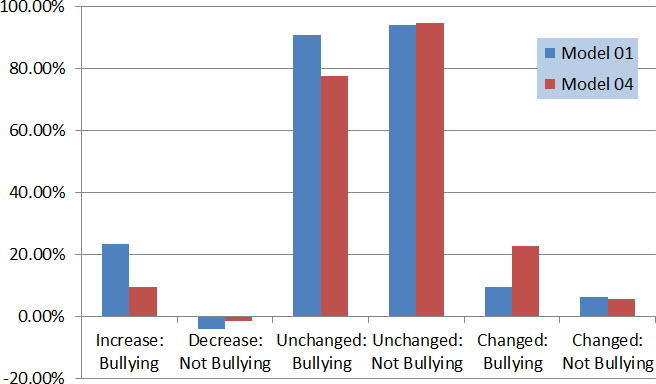
\includegraphics[width=0.75\textwidth]{Figures/Chapter5/scikit_analysis_01.jpg}
	\caption[Percentage change in hold back dataset classification]{Chart showing the percentage change in multiple measures between the two classifications performed on on the hold back data}
	\label{fig:scikit_analysis_01}
\end{figure}

Figure \ref{fig:scikit_analysis_01} can be broken into two parts for further examination. The first analysis considers the \verb|Increase: Bullying| and \verb|Decrease: Not Bullying| columns. These two columns are representative of the change in the number of bullying classifications, and the number of not bullying classifications. The number of samples classified as bullying using both models increased. However, the number of bullying classifications made by \verb|model 01| increased by over 23\%. This represents 150\% growth in excess of \verb|model 04|. Though the percentage decrease in the number of not bullying samples appears less significant, this is caused by an imbalance in the classes. The decrease in the number of not bullying classifications in both classes is reflective of the increase in numbers discussed.

The analysis of columns 3 to 6 in \ref{fig:scikit_analysis_01}, shows how stable the classifications made by each model are, or to look at it another way, by how much the classifications of each model changed between the two runs. Column 3, \verb|Unchanged: Bullying|, and column 5, \verb|Changed: Bullying|, show the number of samples predicted as bullying by \verb|model 01| in both executions. A value of 90.63\% unchanged bullying classifications, and 9.37\% changed, shows that this model is very consistent in the bullying predictions that it makes. On the other hand, \verb|model 04| shows a significantly lower value of 77.51\%. This means that 22.49\% of the bullying predictions \verb|model 04| made in the first run, changed to not bullying after the simulation exercise. Columns 4 and 6, \verb|Unchanged: Not Bullying| and \verb|Changed: Not Bullying| are similar percentages for the samples predicted as not bullying. There is not much to choose from between the two models, with unchanged values of 93.97\% and 94.26\% respectively for \verb|model 01| and \verb|model 04|.

To further analyse the performance of the two models, questions that changed classification were examined. Each question that changed classification was manually classified, in total over 1,600 samples, and then compared to the prediction made by the models. Figure \ref{fig:second_classification} shows the results of this analysis.

\begin{figure}[htbp]
	\centering
	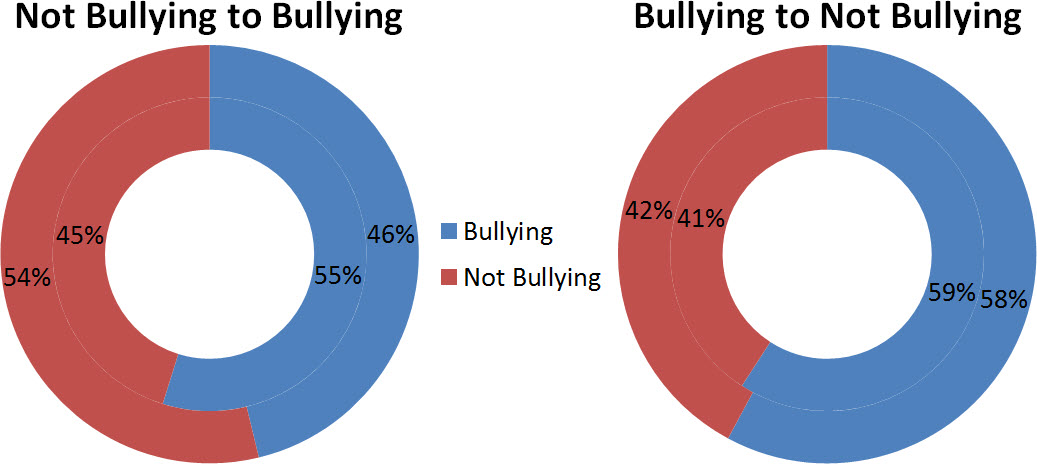
\includegraphics[width=0.75\textwidth]{Figures/Chapter5/second_classification.jpg}
	\caption[Analysis of samples that changed classification]{Graphs showing the percentage of questions that changed classification from bullying to not bullying, and from not bullying to bullying, for the final two models}
	\label{fig:second_classification}
\end{figure}

The doughnut on the left-hand side represents the samples that changed classification from not bullying to bullying. The donut on the right is the samples that changed from bullying to not bullying. The inside ring of each doughnut is \verb|model 01|, the outside ring is \verb|model 04|. Considering the samples that changed from not bullying to bullying first. It is seen that, although neither model excelled, \verb|model 01| correctly reclassified 55\% of questions to bullying. At 59\% and 58\% neither model was very accurate when reclassifying bullying questions as not bullying. It should, however, be noted that \verb|model 01| only reclassified 164 bullying questions, or 1.46\% of all samples, which is a very low percentage. Of these 164 samples there were 67, or 41\%, correctly reclassified.

The final analysis performed on each model was a manual classification of bullying and not bullying samples that did not change classification between the two model executions. The results of this reclassification are shown in Figure \ref{fig:manual_classification}. Once again it is seen that \verb|model 01|, on the inside of each doughnut, has outperformed \verb|model 04| by correctly predicting 92\% of bullying questions, and 87\% of not bullying questions. This model, when originally developed is Section \ref{subsection:scikit-class-imbalance}, had a positive class recall value of 1.000, 100\%, and a negative class recall of 0.904, 90.4\%. So, although the models performance on unseen data was not as good when compared to the values achieved during training, they are still more than satisfactory. 

\begin{figure}[htbp]
	\centering
	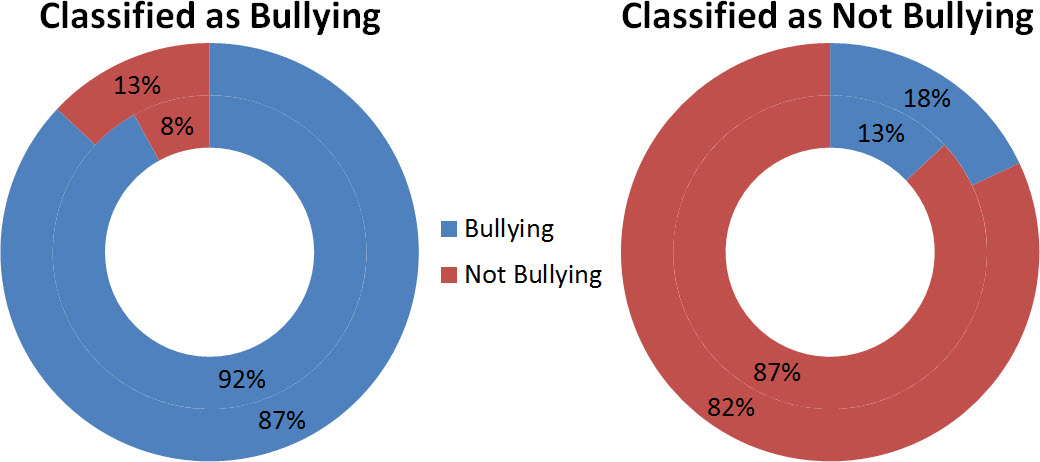
\includegraphics[width=0.75\textwidth]{Figures/Chapter5/manual_classification.jpg}
	\caption[Sample analysis of samples that did not change classification]{Graphs showing the percentage of bullying questions and not bullying question that did not change classification and where the class was correctly predicted}
	\label{fig:manual_classification}
\end{figure}

Of the five models analysed, the model that appears to have performed the best is the scikit-learn support vector model using 1:1 over sampling, stop words included and uni-grams and bi-grams. This model was also considered the best performer of the five model before the automatic evolution of the model using the simulation dataset. This is far from a definitive declaration of the best model. There is significant potential here for future work as discussed in Chapter \ref{chapter6}.